\chapter{Screenshots of the client}
\label{app:clientscreenshots}

\section{Learning process}

\begin{figure}
    \centering
    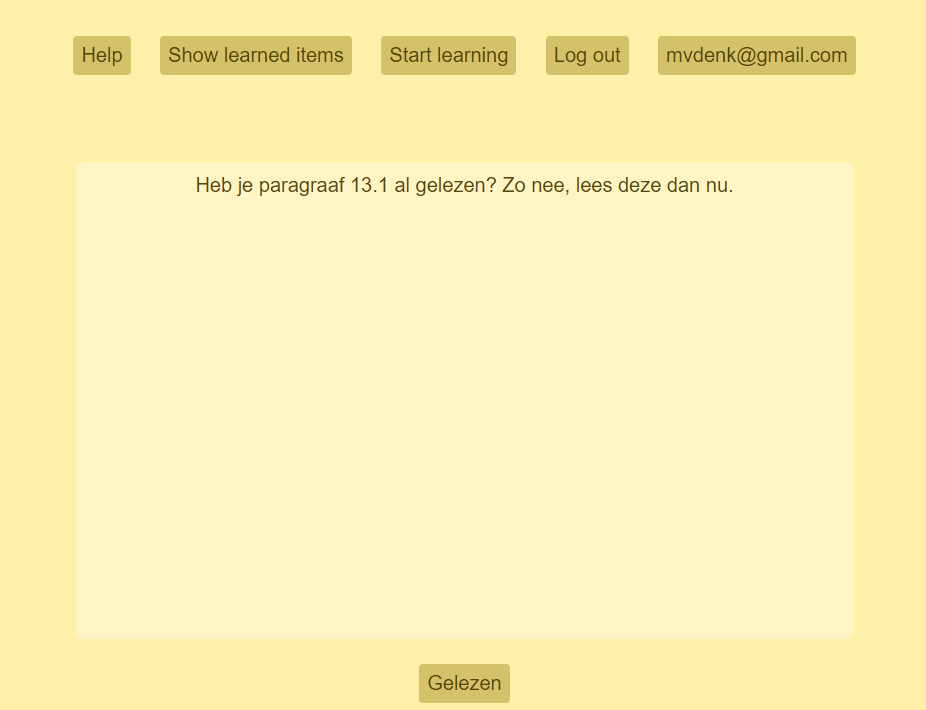
\includegraphics[width=.8\textwidth]{img/ui_read_request.png}
    \caption{The user interface when prompting the user whether he has read paragraph 13.1}
    \label{fig:ui_read_request}
\end{figure}

\begin{figure}
    \centering
    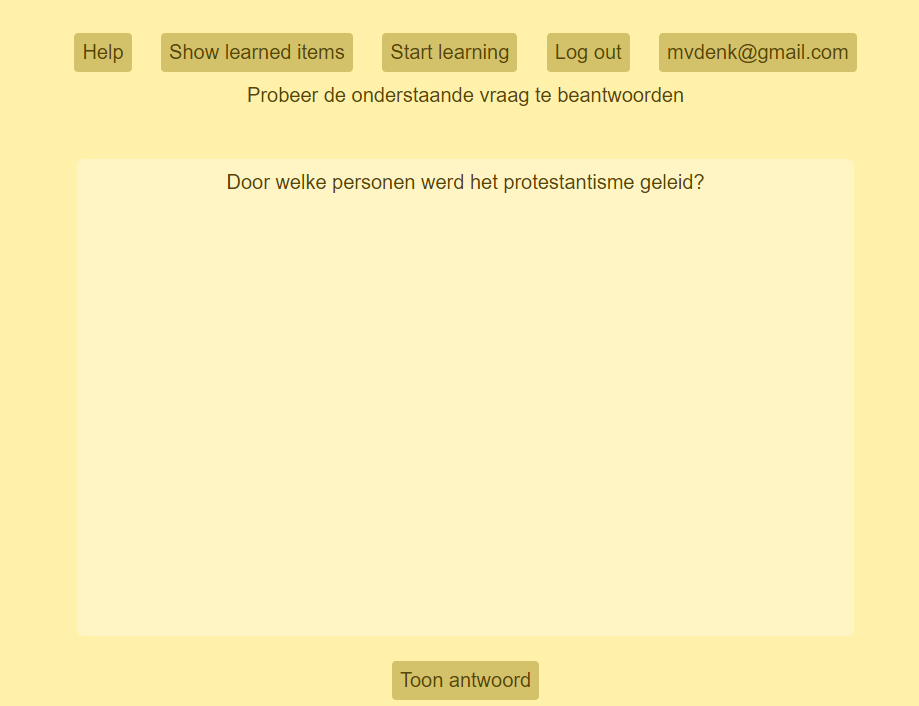
\includegraphics[width=.8\textwidth]{img/ui_fc_prompt.png}
    \caption{The user interface when prompting a flashcard}
    \label{fig:ui_fc_prompt}
\end{figure}

\begin{figure}
    \centering
    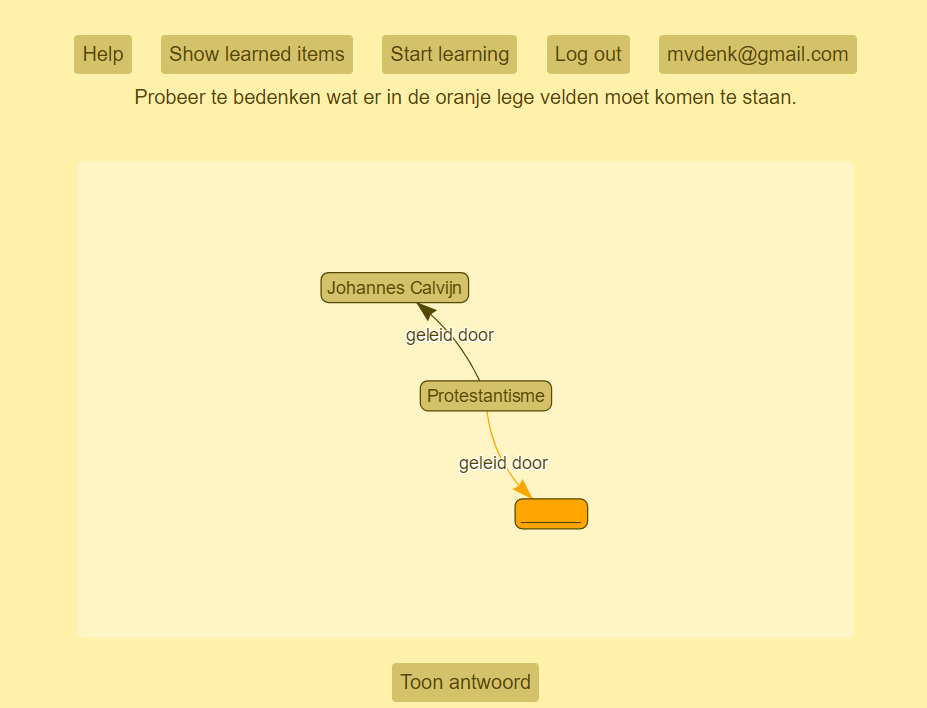
\includegraphics[width=.8\textwidth]{img/ui_fm_prompt.png}
    \caption{The user interface when prompting a flashmap}
    \label{fig:ui_fm_prompt}
\end{figure}

\begin{figure}
    \centering
    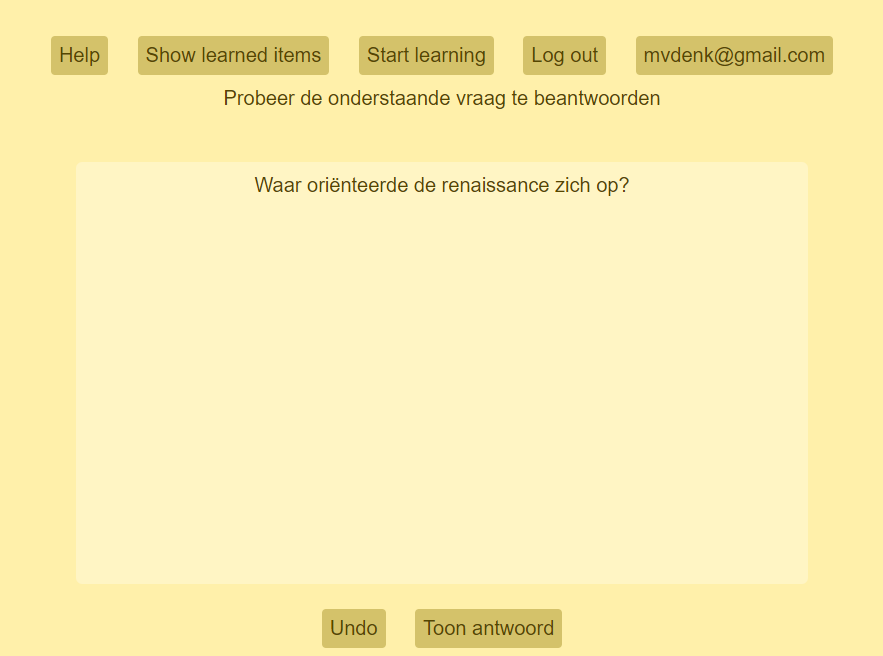
\includegraphics[width=.8\textwidth]{img/ui_undo.png}
    \caption{The user interface when prompting a flashcard with an undo option}
    \label{fig:ui_undo}
\end{figure}

\begin{figure}
    \centering
    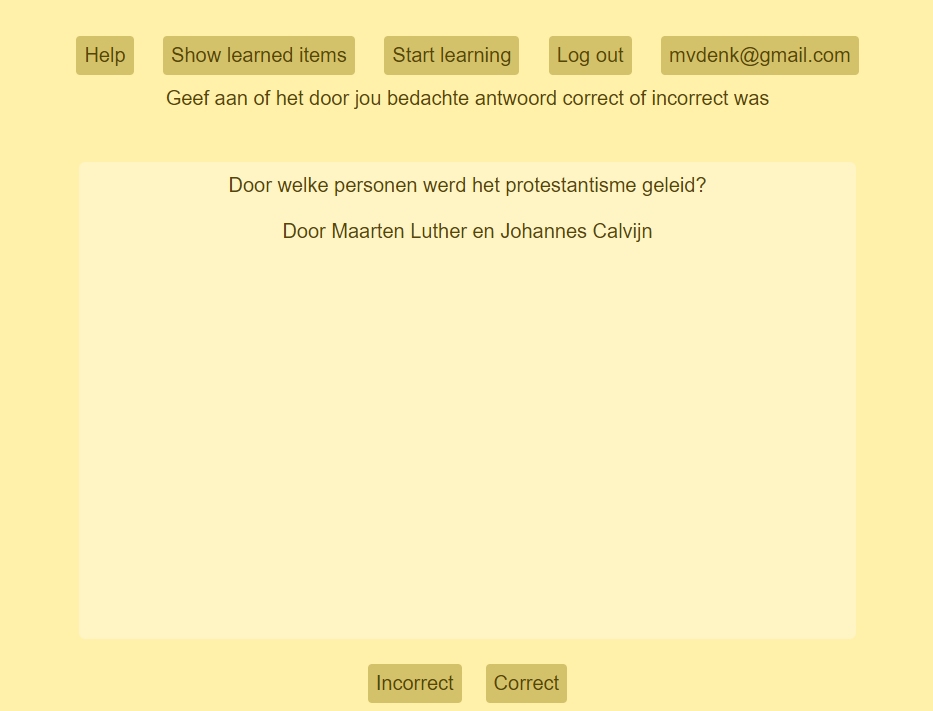
\includegraphics[width=.8\textwidth]{img/ui_fc_answer.png}
    \caption{The user interface when showing the answer to a flashcard}
    \label{fig:ui_fc_answer}
\end{figure}

\begin{figure}
    \centering
    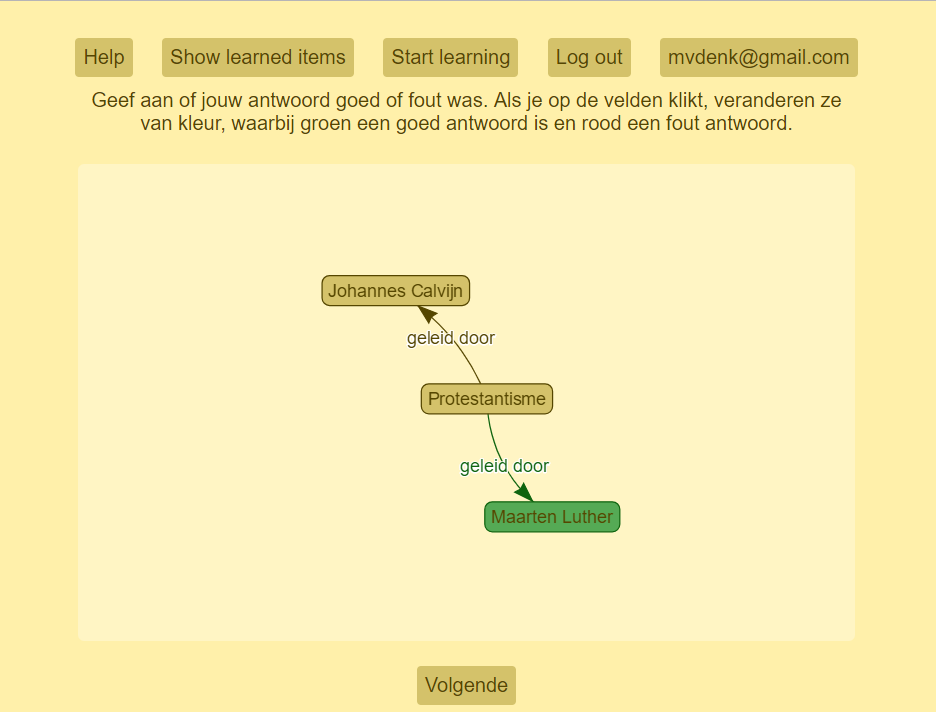
\includegraphics[width=.8\textwidth]{img/ui_fm_answer_correct.png}
    \caption{The user interface when showing the answer to a flashmap, here indicated as correct by the user}
    \label{fig:ui_fm_answer_correct}
\end{figure}

\begin{figure}
    \centering
    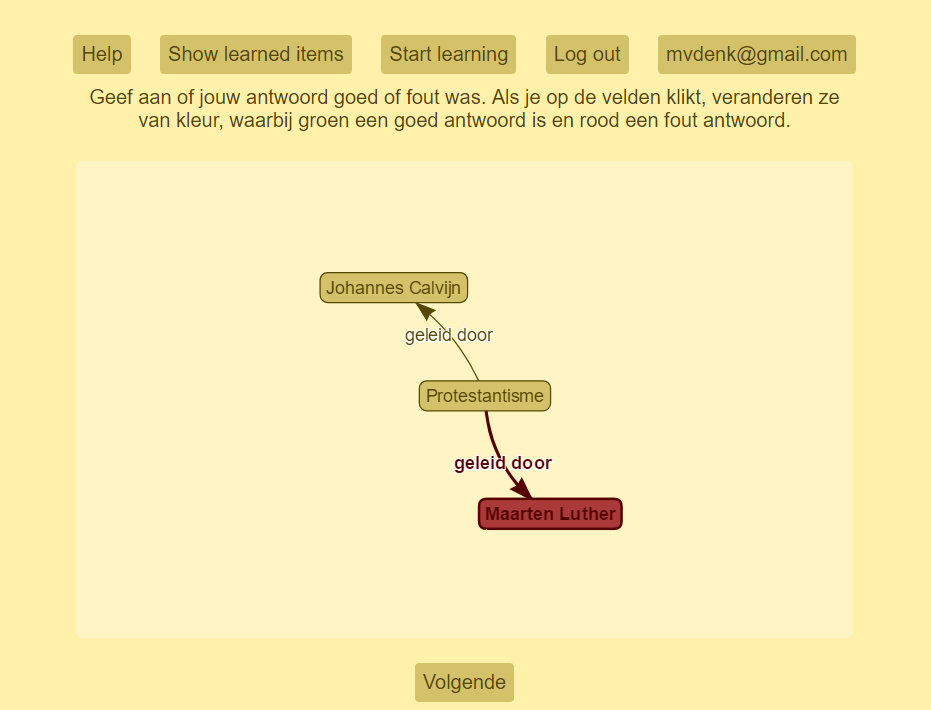
\includegraphics[width=.8\textwidth]{img/ui_fm_answer_incorrect.png}
    \caption{The user interface when showing the answer to a flashmap, here indicated as incorrect by the user}
    \label{fig:ui_fm_answer_incorrect}
\end{figure}

\begin{figure}
    \centering
    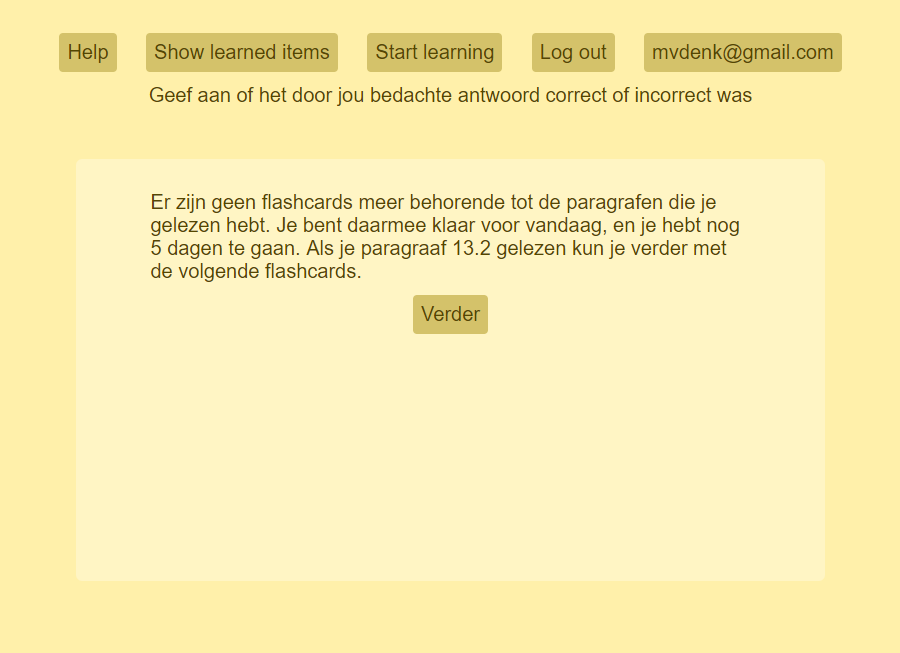
\includegraphics[width=.8\textwidth]{img/ui_no_more_instances.png}
    \caption{The user interface when showing that there are no new instances left to learn}
    \label{fig:ui_no_more_instances}
\end{figure}

\FloatBarrier
\section{Other views}

\begin{figure}
    \centering
    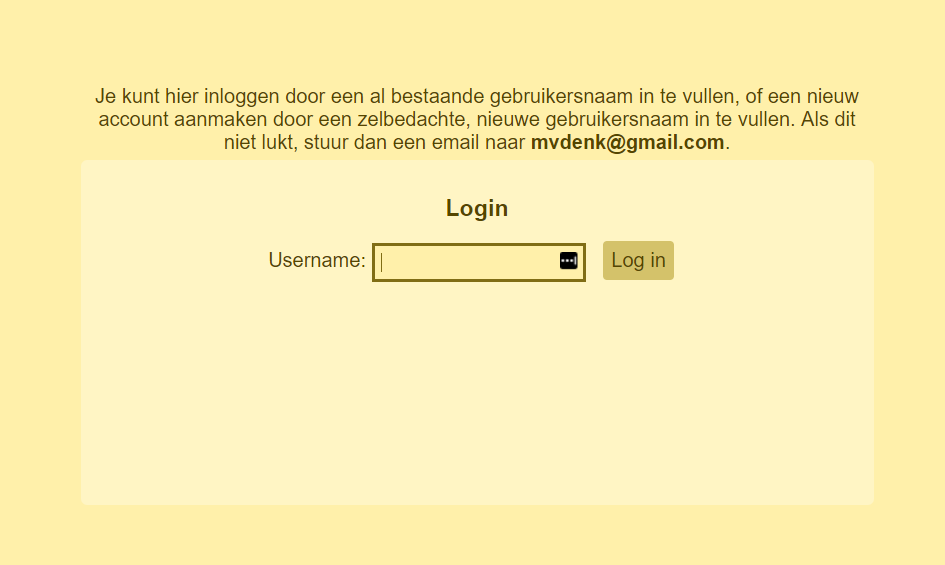
\includegraphics[width=.8\textwidth]{img/ui_login.png}
    \caption{The login screen}
    \label{fig:ui_login}
\end{figure}

\begin{figure}
    \centering
    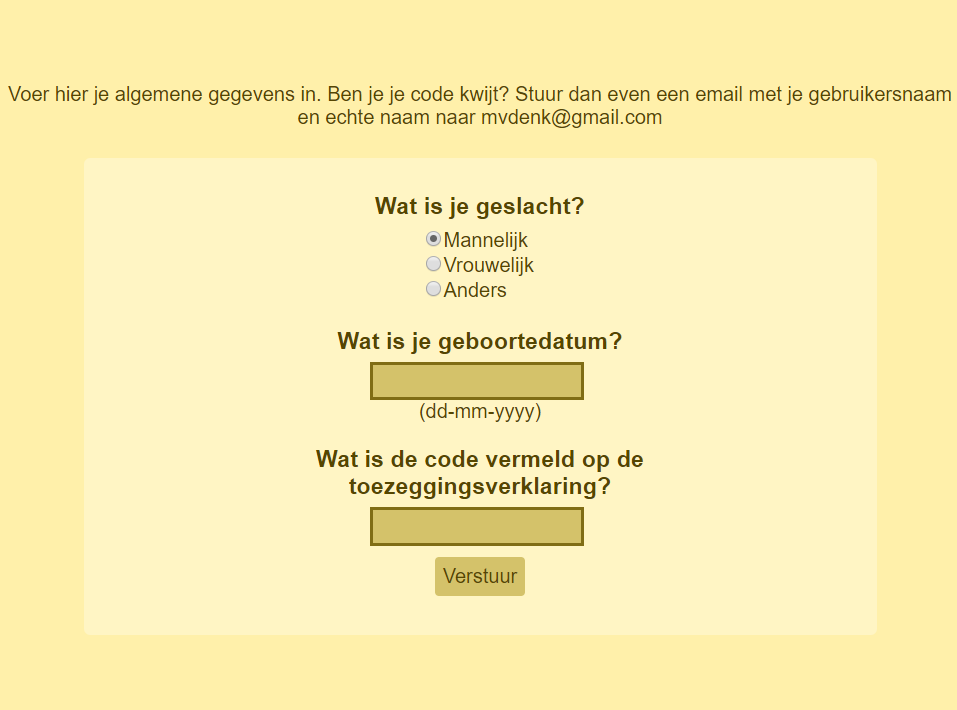
\includegraphics[width=.8\textwidth]{img/ui_descriptives.png}
    \caption{The descriptives screen}
    \label{fig:ui_descriptives}
\end{figure}

\begin{figure}
    \centering
    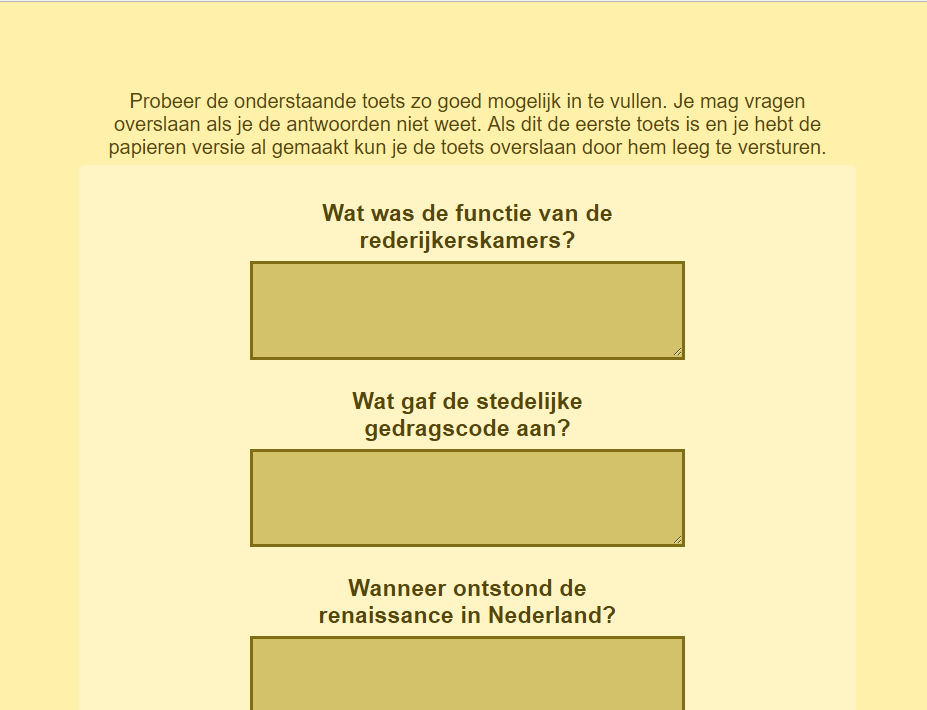
\includegraphics[width=.8\textwidth]{img/ui_test_top.png}
    \caption{The top of the test screen}
    \label{fig:ui_test_top}
\end{figure}

\begin{figure}
    \centering
    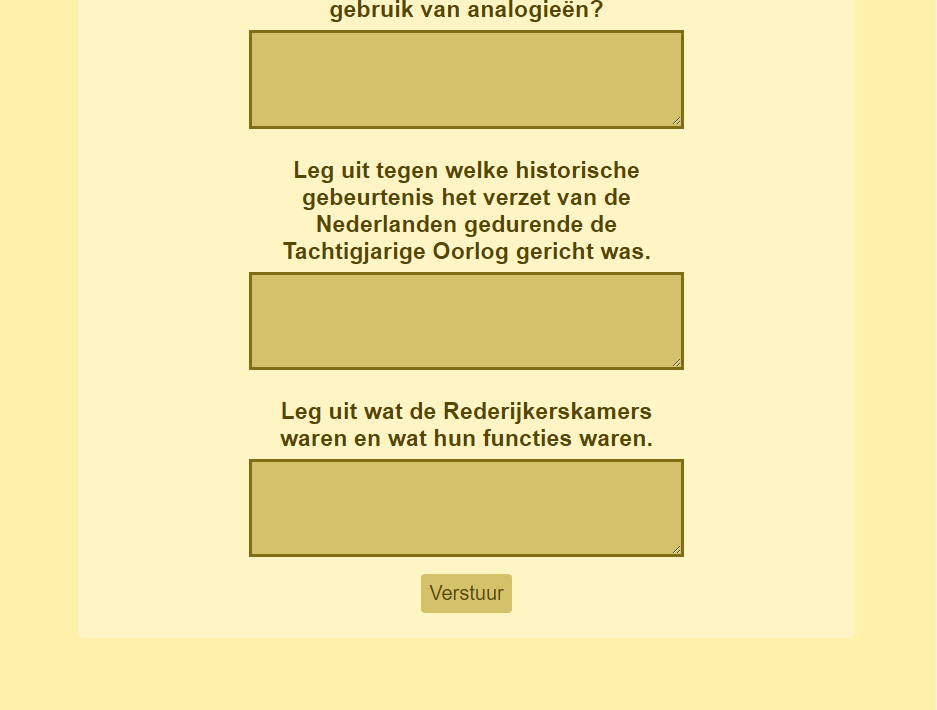
\includegraphics[width=.8\textwidth]{img/ui_test_bottom.png}
    \caption{The bottom of the test screen}
    \label{fig:ui_test_bottom}
\end{figure}

\begin{figure}
    \centering
    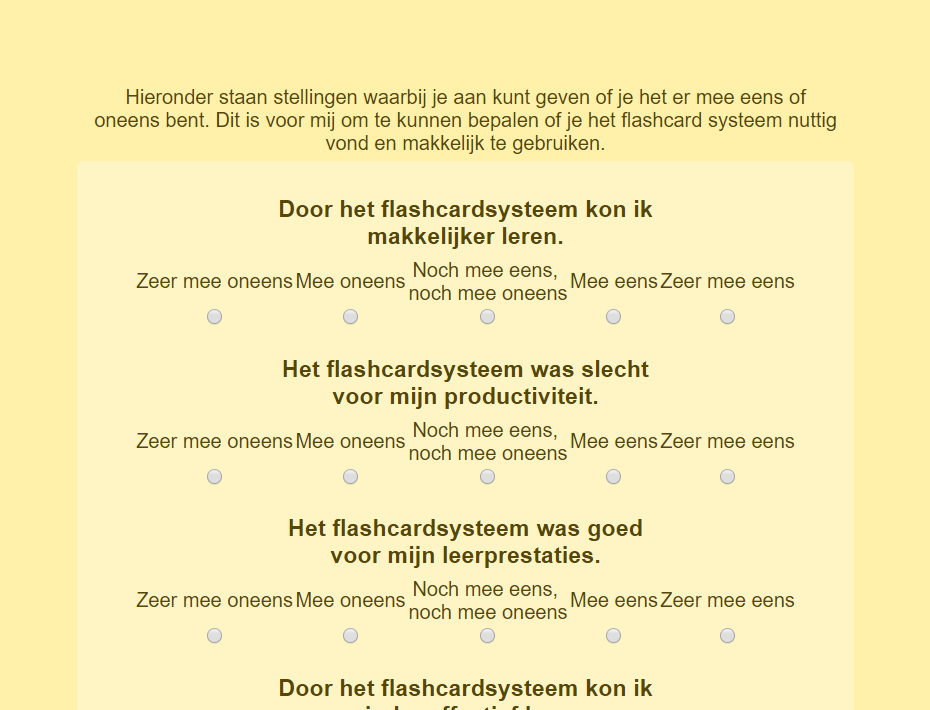
\includegraphics[width=.8\textwidth]{img/ui_questionnaire_top.png}
    \caption{The top of the questionnaire screen}
    \label{fig:ui_questionnaire_top}
\end{figure}

\begin{figure}
    \centering
    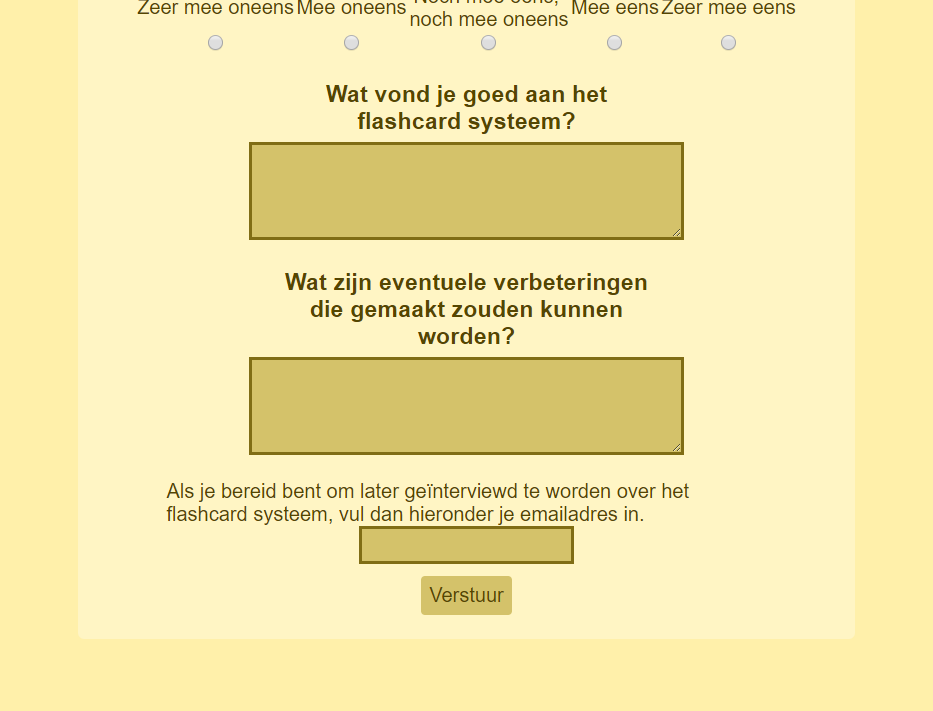
\includegraphics[width=.8\textwidth]{img/ui_questionnaire_bottom.png}
    \caption{The bottom of the questionnaire screen}
    \label{fig:ui_questionnaire_bottom}
\end{figure}

\begin{figure}
    \centering
    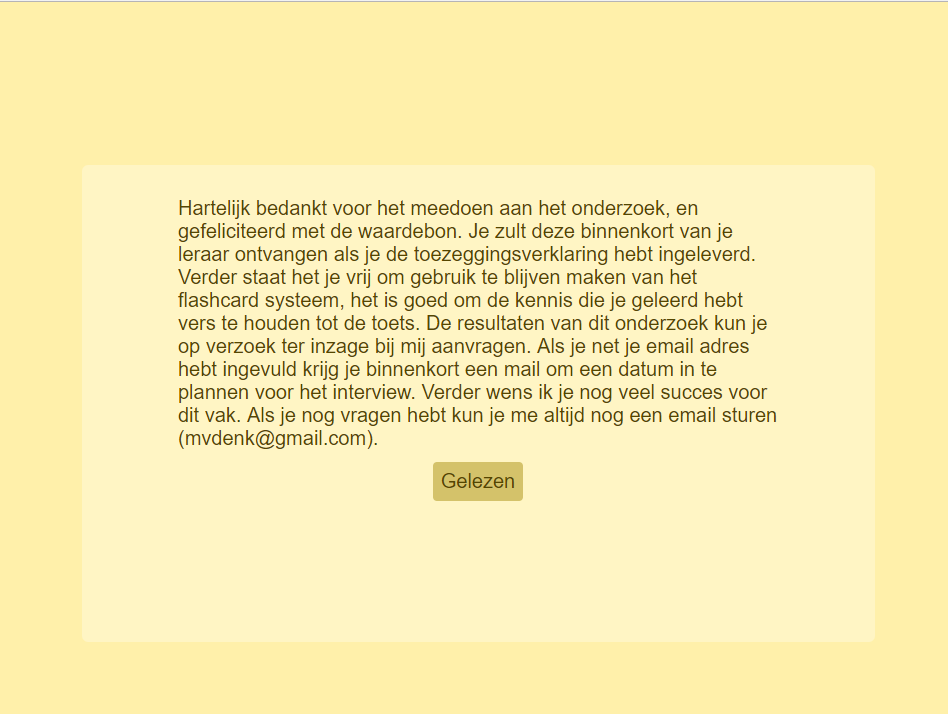
\includegraphics[width=.8\textwidth]{img/ui_debriefing.png}
    \caption{The debriefing screen}
    \label{fig:ui_debriefing}
\end{figure}

\begin{figure}
    \centering
    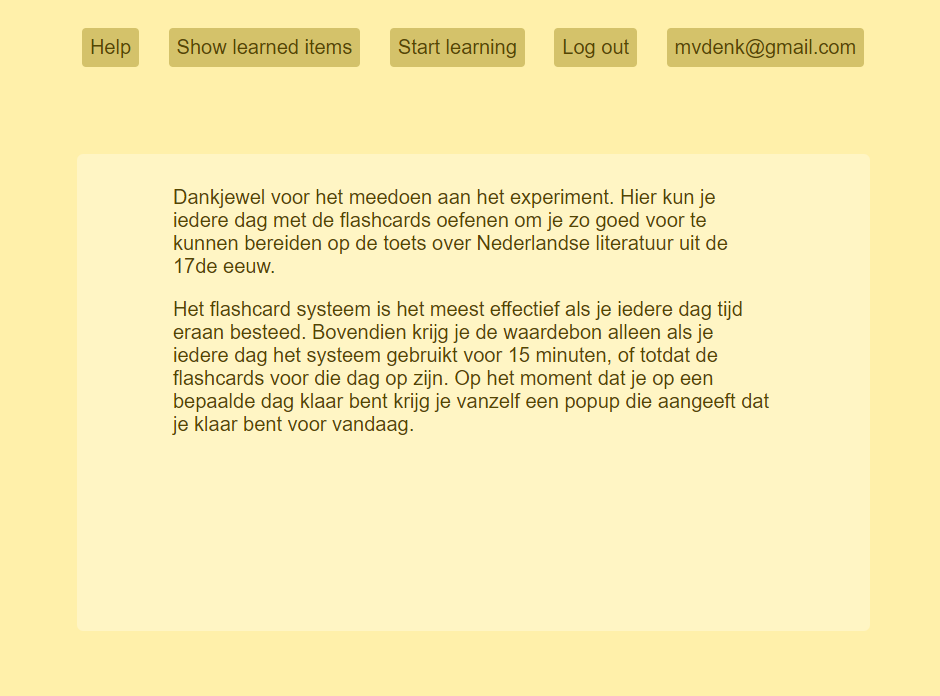
\includegraphics[width=.8\textwidth]{img/ui_help.png}
    \caption{The help screen}
    \label{fig:ui_help}
\end{figure}

\begin{figure}
    \centering
    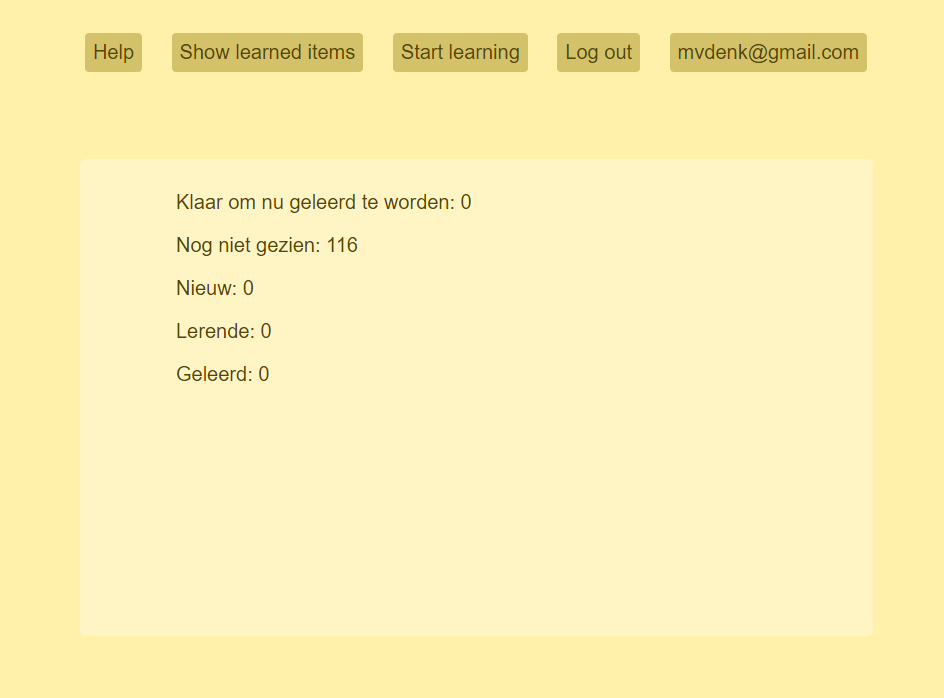
\includegraphics[width=.8\textwidth]{img/ui_fc_learnprogress_1.png}
    \caption{The user interface when showing the learning progress to a flashcard user}
    \label{fig:ui_fc_learnprogress_1}
\end{figure}

\begin{figure}
    \centering
    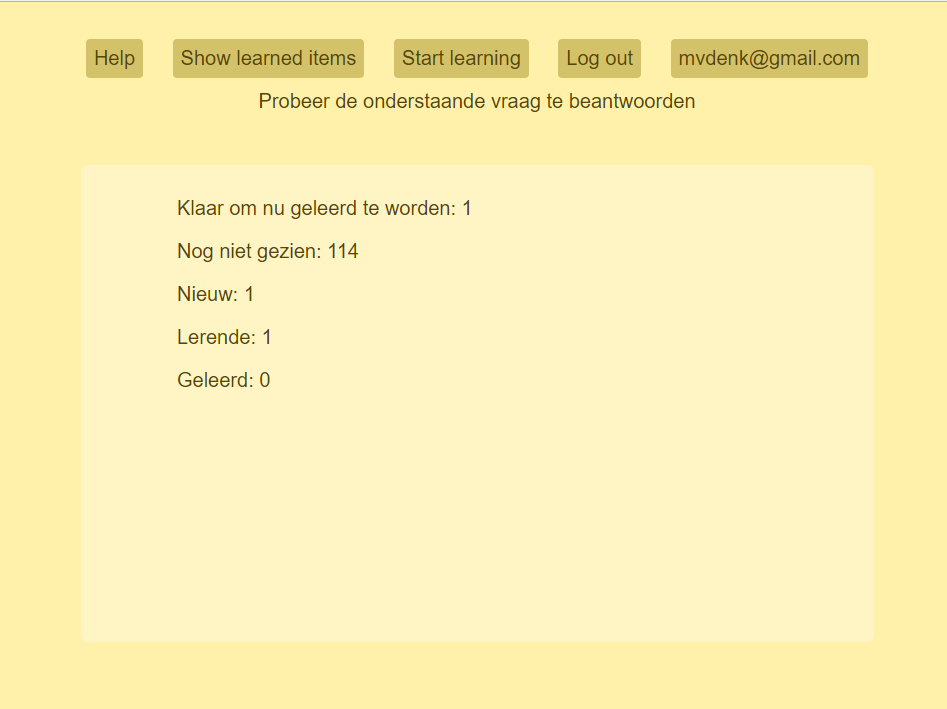
\includegraphics[width=.8\textwidth]{img/ui_fc_learnprogress_2.png}
    \caption{The user interface when showing the learning progress to a flashcard user after reviewing some of the flashcards}
    \label{fig:ui_fc_learnprogress_2}
\end{figure}

\begin{figure}
    \centering
    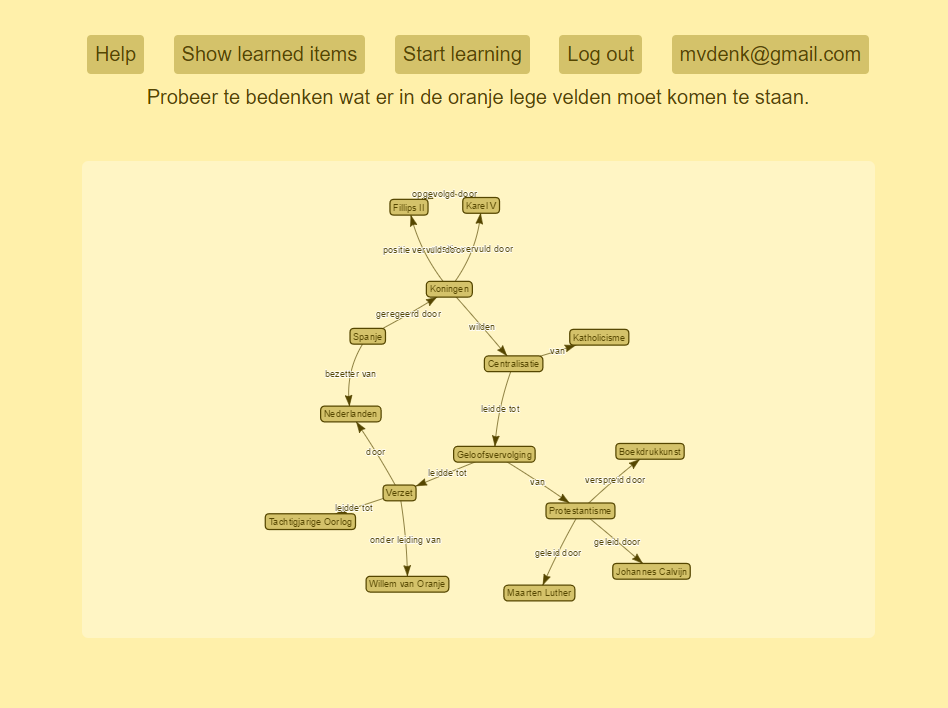
\includegraphics[width=.8\textwidth]{img/ui_fm_learnprogress.png}
    \caption{The user interface when showing the learning progress to a flashmap user}
    \label{fig:ui_fm_learnprogress}
\end{figure}

